\chapter{De voortgangstabel}\label{ch:g10:reaction-progress-table}

% ledger: use:NaN3-airbag
Bij een auto-ongeluk schiet er een kussen uit het stuur, dat zich in een
fractie van een seconde met gas vult, nog voordat het hoofd van de
bestuurder naar voren beweegt. Het gas ontstaat door een \omterm{def:g7:chemical-reactions:reaction}{chemische
reactie}: een kleine lading vaste stof, natriumazide in het klassieke
ontwerp, valt uiteen in natrium en stikstof. De ingenieur moet genoeg
vaste stof gebruiken om het kussen te vullen, maar niet zoveel dat het
knapt, en er mag geen \omterm{def:g7:chemical-reactions:reactant}{beginstof} overblijven die de inzittenden kan
schaden. Hoeveel vaste stof geeft hoeveel gas? Een \omterm{def:g8:balanced-equations:equation}{kloppende
reactievergelijking} geeft de verhoudingen; dit hoofdstuk maakt daar een
boekhoudkundig hulpmiddel van dat elke \omterm{def:g7:chemical-reactions:reactant}{beginstof} en elk \omterm{def:g7:chemical-reactions:reactant}{reactieproduct}
volgt van het begin van een reactie tot het einde.

\begin{recall}
Een \omterm{def:g8:balanced-equations:equation}{kloppende reactievergelijking} houdt het aantal \omterm{def:g7:atoms-and-molecules:atom}{atomen} van elk
element, en de lading, aan beide kanten gelijk; de \omterm{def:g8:balanced-equations:coefficient}{coëfficiënten} geven
de verhoudingen waarin de stoffen reageren
(\cref{ch:g8:balanced-equations}). De hoeveelheid van een stof is
$n = m/M$ voor een massa, $n = V/V_m$ voor een gas (met
$V_m = \qty{24.1}{L/mol}$ bij \qty{20}{\celsius} en normale atmosferische
druk) (\cref{ch:g10:the-mole}), en $n = c \times V$ voor een \omterm{def:g6:solutions-and-solubility:solute}{opgeloste
stof} (\cref{ch:g10:concentration-and-dilution}).
\end{recall}

\begin{omfigure}
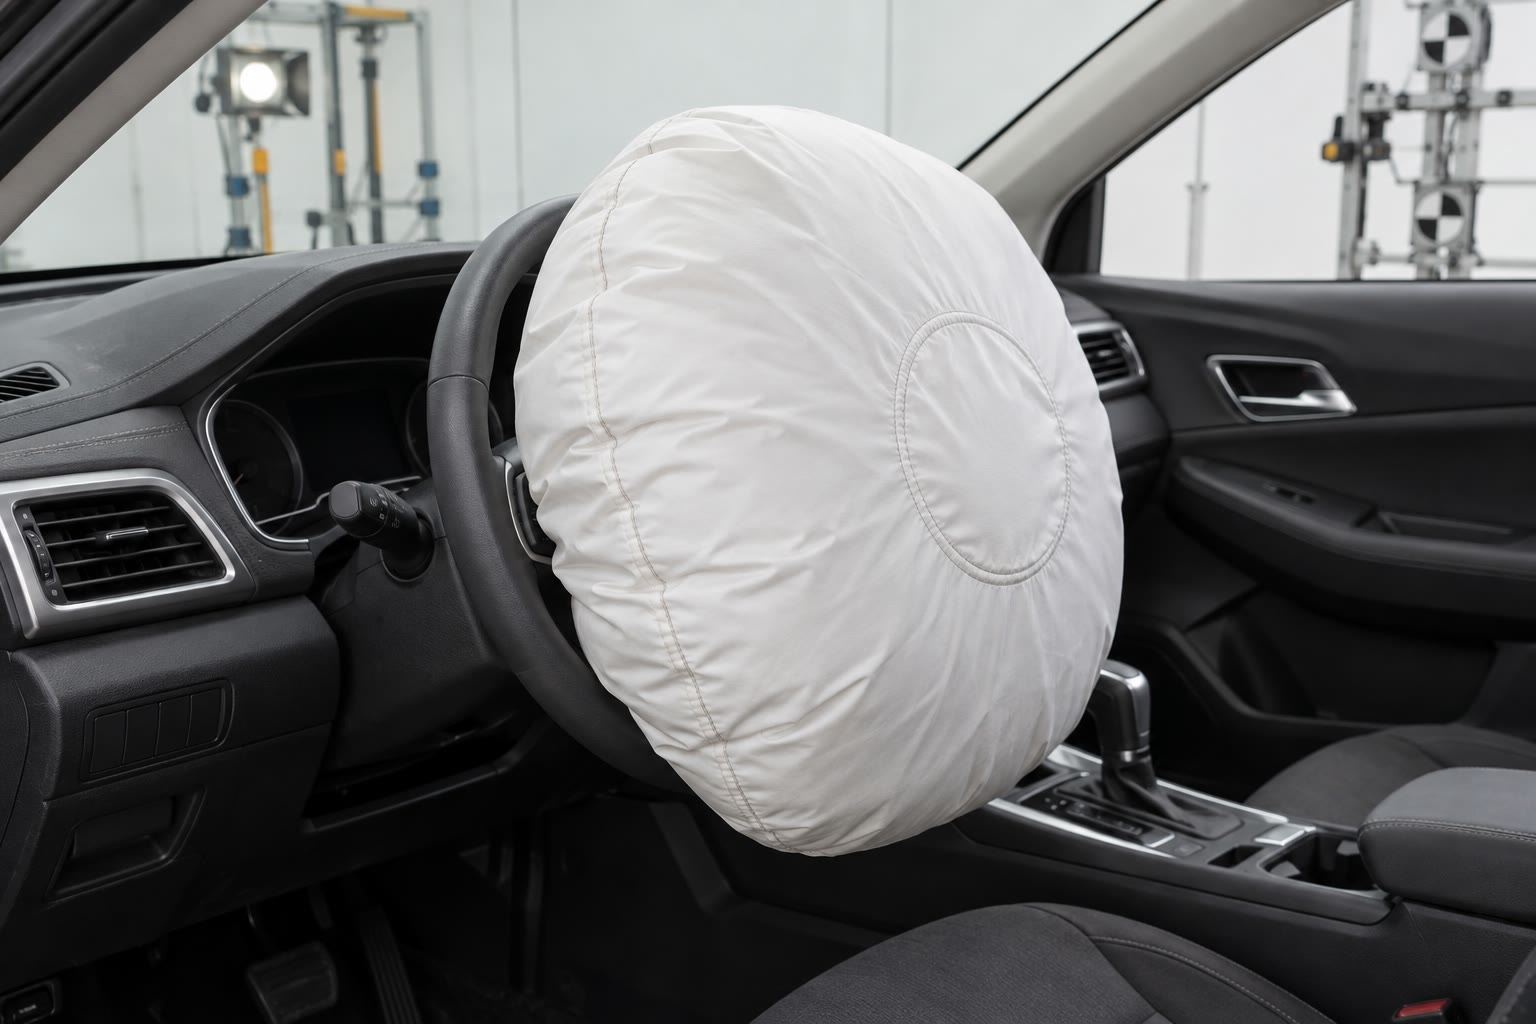
\includegraphics[width=0.5\linewidth]{images/book1/ai/g10-airbag.jpg}

{\small Een airbag vult zich in een fractie van een seconde met de
stikstof die een reactie maakt.}
\end{omfigure}

\section{Een chemisch systeem beschrijven}

\begin{definition}[Chemisch systeem, begin- en eindtoestand]\label{def:g10:reaction-progress-table:system}
Een \emph{chemisch systeem}\index{chemisch systeem} is het geheel van
\omterm{def:g6:pure-substances-and-mixtures:species}{chemische stoffen} dat op een bepaalde plaats aanwezig is (een kolf, een
kussen, een cel), elk met zijn hoeveelheid en zijn fysische toestand. Het
systeem voordat de reactie begint, is de
\emph{begintoestand}\index{begintoestand}; het systeem nadat de reactie
gestopt is, is de \emph{eindtoestand}\index{eindtoestand}.
\end{definition}


\begin{example}[Methaan dat in een gesloten vat verbrandt]\label{ex:g10:reaction-progress-table:methane}
Een gesloten vat bevat \qty{2.0}{mol} methaan en \qty{3.0}{mol}
zuurstof; een vonk zet de \omterm{def:g4:what-a-fire-needs:burning}{verbranding}
\ce{CH4 + 2O2 -> CO2 + 2H2O} in gang. In de \omterm{def:g10:reaction-progress-table:system}{begintoestand} bevat het
systeem \qty{2.0}{mol} \ce{CH4(g)}, \qty{3.0}{mol} \ce{O2(g)} en geen
\omterm{def:g7:chemical-reactions:reactant}{reactieproducten}. Wat zit er in de \omterm{def:g10:reaction-progress-table:system}{eindtoestand}? De rest van het
hoofdstuk geeft het antwoord.
\end{example}

\section{De reactievoortgang en de voortgangstabel}

\begin{definition}[Reactievoortgang, voortgangstabel]\label{def:g10:reaction-progress-table:extent}
De \emph{reactievoortgang}\index{reactievoortgang} $x$, in \omterm{def:g10:the-mole:amount}{mol}, telt hoe
vaak de reactie, zoals geschreven in de \omterm{def:g8:balanced-equations:equation}{kloppende reactievergelijking},
heeft plaatsgevonden: bij een voortgang $x$ is van een stof met
\omterm{def:g8:balanced-equations:coefficient}{coëfficiënt} $\nu$ de hoeveelheid $\nu x$ verbruikt (\omterm{def:g7:chemical-reactions:reactant}{beginstof}) of
gevormd (\omterm{def:g7:chemical-reactions:reactant}{reactieproduct}). De
\emph{voortgangstabel}\index{voortgangstabel} geeft onder de
vergelijking de hoeveelheid van elke stof in de \omterm{def:g10:reaction-progress-table:system}{begintoestand}, bij een
voortgang $x$, en in de \omterm{def:g10:reaction-progress-table:system}{eindtoestand}.
\end{definition}

\begin{method}[Een voortgangstabel invullen]\label{met:g10:reaction-progress-table:fill}
\begin{enumerate}
  \item Schrijf de \omterm{def:g8:balanced-equations:equation}{kloppende reactievergelijking} in de eerste rij.
  \item \omterm{def:g10:reaction-progress-table:system}{Begintoestand} ($x = 0$): schrijf de beginhoeveelheid van elke
        stof eronder.
  \item Tussentoestand (voortgang $x$): elke \omterm{def:g7:chemical-reactions:reactant}{beginstof} met \omterm{def:g8:balanced-equations:coefficient}{coëfficiënt}
        $\nu$ wordt $n_0 - \nu x$, elk \omterm{def:g7:chemical-reactions:reactant}{reactieproduct} $n_0 + \nu x$.
  \item \omterm{def:g10:reaction-progress-table:system}{Eindtoestand}: bepaal $x_{\max}$ (volgende paragraaf) en vul die
        in in de uitdrukkingen van de tussenrij.
\end{enumerate}
\end{method}

\begin{omfigure}
\renewcommand{\arraystretch}{1.25}
\begin{tabular}{l|c|cccc}
\hline
vergelijking & & \ce{CH4} & $+$ \ce{2O2} & $\longrightarrow$ \ce{CO2} & $+$ \ce{2H2O} \\
\hline
toestand & voortgang (\si{mol}) & \multicolumn{4}{c}{hoeveelheden (\si{mol})} \\
\hline
begin & $0$ & $2.0$ & $3.0$ & $0$ & $0$ \\
tussen & $x$ & $2.0 - x$ & $3.0 - 2x$ & $x$ & $2x$ \\
eind & $x_{\max} = 1.5$ & $0.5$ & $0$ & $1.5$ & $3.0$ \\
\hline
\end{tabular}\par\medskip

{\small De \omterm{def:g10:reaction-progress-table:extent}{voortgangstabel} van de \omterm{def:g4:what-a-fire-needs:burning}{verbranding} van methaan uit het
voorbeeld. Elke kolom volgt één stof; de \omterm{def:g8:balanced-equations:coefficient}{coëfficiënten} 2 van \ce{O2} en
van \ce{H2O} worden de $2x$.}
\end{omfigure}

\section{De beperkende beginstof en de eindtoestand}

\begin{definition}[Beperkende beginstof, maximale voortgang, aflopende reactie]\label{def:g10:reaction-progress-table:limiting}
Een reactie is een \emph{aflopende reactie}\index{aflopende reactie} als
ze pas stopt wanneer een van haar \omterm{def:g7:chemical-reactions:reactant}{beginstoffen} op is. Die \omterm{def:g7:chemical-reactions:reactant}{beginstof} is
de \emph{beperkende beginstof}\index{beperkende beginstof}; de andere
\omterm{def:g7:chemical-reactions:reactant}{beginstoffen} zijn in overmaat. De voortgang waarbij de beperkende
\omterm{def:g7:chemical-reactions:reactant}{beginstof} op raakt, is de \emph{maximale voortgang}\index{maximale voortgang}
$x_{\max}$; de \omterm{def:g10:reaction-progress-table:system}{eindtoestand} van een aflopende reactie is de toestand bij
$x = x_{\max}$.
\end{definition}

\begin{method}[De beperkende beginstof vinden]\label{met:g10:reaction-progress-table:limiting}
\begin{enumerate}
  \item Los voor elke \omterm{def:g7:chemical-reactions:reactant}{beginstof} $n_0 - \nu x = 0$ op: de \omterm{def:g7:chemical-reactions:reactant}{beginstof} zou op
        zijn bij $x = n_0 / \nu$.
  \item De kleinste van deze waarden is $x_{\max}$; de \omterm{def:g7:chemical-reactions:reactant}{beginstof} die haar
        geeft, is de \omterm{def:g10:reaction-progress-table:limiting}{beperkende beginstof}.
  \item Vul $x_{\max}$ in in de tussenrij om de \omterm{def:g10:reaction-progress-table:system}{eindtoestand} te krijgen;
        controleer dat geen enkele hoeveelheid negatief is.
\end{enumerate}
\end{method}

\begin{example}[Terug naar het methaan]\label{ex:g10:reaction-progress-table:methane-final}
Methaan zou op zijn bij $x = 2.0/1 = \qty{2.0}{mol}$, zuurstof bij
$x = 3.0/2 = \qty{1.5}{mol}$. De kleinste is \qty{1.5}{mol}: zuurstof is
de \omterm{def:g10:reaction-progress-table:limiting}{beperkende beginstof} en $x_{\max} = \qty{1.5}{mol}$. De \omterm{def:g10:reaction-progress-table:system}{eindtoestand}
bevat \qty{0.5}{mol} overgebleven methaan, geen zuurstof,
\qty{1.5}{mol} koolstofdioxide en \qty{3.0}{mol} water.
\end{example}

\begin{omfigure}
\begin{tikzpicture}
\begin{axis}[width=0.78\linewidth, height=6.2cm, xmin=0, xmax=2.05,
    ymin=0, ymax=4.2, xlabel={voortgang $x$ (\si{mol})},
    ylabel={hoeveelheid (\si{mol})}, axis lines*=left, ymajorgrids,
    grid style={gray!20}, tick label style={font=\small},
    label style={font=\small}, xtick={0,0.5,1,1.5,2},
    legend style={font=\small, at={(1.02,0.5)}, anchor=west, draw=none},
    legend cell align=left]
  \addplot[very thick, omDef, domain=0:2] {2-x};
  \addplot[very thick, omThm, domain=0:1.5] {3-2*x};
  \addplot[very thick, omMeth, domain=0:2] {x};
  \addplot[very thick, omProp, domain=0:2] {2*x};
  \legend{\ce{CH4}, \ce{O2}, \ce{CO2}, \ce{H2O}}
  \addplot[dashed, black!60] coordinates {(1.5,0) (1.5,4.2)};
  \node[font=\small, anchor=south west] at (axis cs:1.5,3.55) {$x_{\max}$};
  \fill[black!8, opacity=0.6] (axis cs:1.5,0) rectangle (axis cs:2.05,4.2);
\end{axis}
\end{tikzpicture}

{\small Hoeveelheden uitgezet tegen de voortgang voor het voorbeeld met
methaan. Zuurstof (rood) bereikt als eerste nul, bij $x = \qty{1.5}{mol}$:
daar stopt de reactie, en het gearceerde deel wordt nooit bereikt.}
\end{omfigure}

\begin{remark}[Niet alle reacties zijn aflopend]\label{rem:g10:reaction-progress-table:not-total}
Veel reacties stoppen voordat er een \omterm{def:g7:chemical-reactions:reactant}{beginstof} op is: ze bereiken een
toestand waarin \omterm{def:g7:chemical-reactions:reactant}{beginstoffen} en \omterm{def:g7:chemical-reactions:reactant}{reactieproducten} naast elkaar bestaan.
Hun \omterm{def:g10:reaction-progress-table:system}{eindtoestand} is niet $x_{\max}$, en een later hoofdstuk leert die te
bepalen. In dit hoofdstuk is elke reactie aflopend.
\end{remark}

\section{Het stoichiometrisch mengsel}

\begin{definition}[Stoichiometrisch mengsel]\label{def:g10:reaction-progress-table:stoichiometric}
Een \omterm{def:g6:pure-substances-and-mixtures:mixture}{mengsel} van \omterm{def:g7:chemical-reactions:reactant}{beginstoffen} is een \emph{stoichiometrisch
mengsel}\index{stoichiometrisch mengsel} als de beginhoeveelheden in de
verhouding staan van de \omterm{def:g8:balanced-equations:coefficient}{coëfficiënten} van de \omterm{def:g8:balanced-equations:equation}{kloppende
reactievergelijking}.
\end{definition}

\begin{proposition}[Alle beginstoffen raken tegelijk op]\label{prop:g10:reaction-progress-table:together}
Voor een reactie $a\,\ce{A} + b\,\ce{B} \longrightarrow$ producten is het \omterm{def:g6:pure-substances-and-mixtures:mixture}{mengsel} stoichiometrisch dan en
slechts dan als
\[
  \frac{n_0(\ce{A})}{a} = \frac{n_0(\ce{B})}{b},
\]
en dan zijn bij een \omterm{def:g10:reaction-progress-table:limiting}{aflopende reactie} in de \omterm{def:g10:reaction-progress-table:system}{eindtoestand} beide
\omterm{def:g7:chemical-reactions:reactant}{beginstoffen} verbruikt.
\end{proposition}

\begin{proof}
\ce{A} zou op zijn bij $x = n_0(\ce{A})/a$, \ce{B} bij $x = n_0(\ce{B})/b$.
De twee waarden zijn precies gelijk als de verhoudingen die van de
vergelijking zijn, en dan maakt de voortgang $x_{\max}$ beide tegelijk
op.
\end{proof}

\begin{example}[Methaan schoon verbranden]\label{ex:g10:reaction-progress-table:stoich}
Voor \ce{CH4 + 2O2 -> CO2 + 2H2O} heeft \qty{2.0}{mol} methaan
\qty{4.0}{mol} zuurstof nodig: $2.0/1 = 4.0/2$. Met maar \qty{3.0}{mol}
zuurstof had het \omterm{def:g6:pure-substances-and-mixtures:mixture}{mengsel} uit het eerste voorbeeld te weinig zuurstof; in
een echte vlam is het juist dat tekort dat het giftige koolstofmono-oxide
maakt (\cref{ch:g8:combustion-and-fuels}).
\end{example}

\section{Gassen en oplossingen in de tabel}


\begin{method}[Hoeveelheden voor de begintoestand]\label{met:g10:reaction-progress-table:amounts}
Reken voordat je een tabel invult elke gegeven grootheid om naar een
hoeveelheid: $n = m/M$ voor een gewogen vaste stof of vloeistof;
$n = V/V_m$ voor een gas; $n = c \times V$ voor een \omterm{def:g6:solutions-and-solubility:solute}{opgeloste stof}. Reken
aan het eind de hoeveelheden van de \omterm{def:g10:reaction-progress-table:system}{eindtoestand} weer om naar wat er
gevraagd wordt: massa, gasvolume of concentratie.
\end{method}

\begin{example}[Magnesium in zoutzuur]\label{ex:g10:reaction-progress-table:magnesium}
% ledger: aw:Mg
Zoutzuur bevat waterstofionen \ce{H+}, die magnesium aantasten:
\ce{Mg + 2H+ -> Mg^{2+} + H2}. Een lintje van \qty{0.12}{g} magnesium
wordt in \qty{50.0}{mL} zuur gegooid met $c(\ce{H+}) = \qty{1.0}{mol/L}$.
Beginhoeveelheden: $n_0(\ce{Mg}) = 0.12/24.3 = \qty{4.9e-3}{mol}$ en
$n_0(\ce{H+}) = 1.0 \times 0.0500 = \qty{5.0e-2}{mol}$. Magnesium zou op
zijn bij $x = \qty{4.9e-3}{mol}$, de waterstofionen bij
$x = 0.050/2 = \qty{2.5e-2}{mol}$: magnesium is beperkend en
$x_{\max} = \qty{4.9e-3}{mol}$. De reactie geeft \qty{4.9e-3}{mol}
waterstof, dat is $\num{4.9e-3} \times 24.1 = \qty{0.12}{L}$ bij
\qty{20}{\celsius}, en laat $0.050 - 2 \times 0.0049 =
\qty{0.040}{mol}$ waterstofionen in overmaat achter.
\end{example}

\begin{inthelab}[Ballonnen op kolven]
De docent giet \qty{50.0}{mL} van hetzelfde zoutzuur in elk van zes
erlenmeyers, en doet in zes ballonnen toenemende massa's
magnesiumpoeder: 0.15, 0.30, 0.45, 0.60, 0.75 en \qty{0.90}{g}. Elke
ballon wordt over de hals van zijn erlenmeyer getrokken en dan opgetild,
zodat het poeder in het zuur valt. Bruisend zwellen de ballonnen op. Als
alles gestopt is, zijn de ballonnen van de eerste tot de vierde kolf
steeds groter; de vierde, vijfde en zesde zijn even groot, en in de
laatste twee ligt nog wat grijs poeder op de bodem van de kolf.
\end{inthelab}

\begin{omfigure}
\begin{tikzpicture}[font=\small, scale=0.82]
  % H2 volume (L): 0.149 0.298 0.446 0.595 0.6025 0.6025; radius ~ V^(1/3)
  \foreach \i/\m/\v/\r/\left in {0/0.15/0.15/0.42/0, 1/0.30/0.30/0.53/0,
      2/0.45/0.45/0.61/0, 3/0.60/0.60/0.67/0, 4/0.75/0.60/0.67/1,
      5/0.90/0.60/0.67/1} {
    \begin{scope}[shift={(2.35*\i,0)}]
      \pic[transform shape] at (0,0) {erlenmeyer={0.25}{omWater}};
      \ifnum\left=1
        \fill[black!45] (-0.5,0.03) rectangle (0.5,0.12);
      \fi
      \fill[omProp!35, draw=omProp!80!black] (-0.3,2.6) -- (0.3,2.6)
        -- (0.12,2.82) -- (-0.12,2.82) -- cycle;
      \shade[ball color=omProp!40, draw=omProp!80!black]
        (0,{2.78+\r}) circle (\r);
      \node[align=center, anchor=north] at (0,-0.15)
        {\qty{\m}{g} Mg\\ \qty{\v}{L}};
    \end{scope}
  }
\end{tikzpicture}

{\small Zes erlenmeyers met hetzelfde zuur en steeds meer magnesium, met
het volume waterstof (bij \qty{20}{\celsius}) in elke ballon. Boven
ongeveer \qty{0.61}{g} is het zuur beperkend: de ballonnen groeien niet
meer en er blijft magnesium over (grijs).}
\end{omfigure}

\begin{remark}[Het plateau aflezen]\label{rem:g10:reaction-progress-table:plateau}
In de eerste kolven is magnesium de \omterm{def:g10:reaction-progress-table:limiting}{beperkende beginstof}, en als je het
verdubbelt, verdubbelt het gas. Vanaf een bepaalde massa raken de
waterstofionen als eerste op: meer magnesium verandert dan alleen nog
het overgebleven poeder. De omslag ligt precies bij het
\omterm{def:g10:reaction-progress-table:stoichiometric}{stoichiometrische mengsel},
$n_0(\ce{Mg}) = n_0(\ce{H+})/2 = \qty{0.025}{mol}$, dat is
$0.025 \times 24.3 = \qty{0.61}{g}$ magnesium.
\end{remark}

\begin{safety}{\ghs[0.82cm]{GHS02}\ghs[0.82cm]{GHS05}\ghs[0.82cm]{GHS07}}
% ledger: ghs:Mg, ghs:HCl
Magnesiumpoeder is ontvlambaar; zoutzuur verbrandt de huid en de ogen en
de dampen irriteren de luchtwegen; waterstof brandt in \omterm{def:g4:air-a-mixture-of-gases:air}{lucht}. Een
demonstratie door de docent, met veiligheidsbril, ver van elke vlam.
\end{safety}

\section{Oefeningen}

\begin{exercise}[$\star$]\label{exo:g10:reaction-progress-table:1}
Vul de \omterm{def:g10:reaction-progress-table:extent}{voortgangstabel} in van \ce{2H2 + O2 -> 2H2O} voor een
beginmengsel van \qty{4.0}{mol} waterstof en \qty{3.0}{mol} zuurstof,
aangenomen dat de reactie aflopend is. Geef $x_{\max}$, de \omterm{def:g10:reaction-progress-table:limiting}{beperkende
beginstof} en de \omterm{def:g10:reaction-progress-table:system}{eindtoestand}.
\end{exercise}

\begin{exercise}[$\star$]\label{exo:g10:reaction-progress-table:2}
Koolstof verbrandt in zuurstof: \ce{C + O2 -> CO2}. Bepaal, uitgaande van
\qty{3.0}{mol} koolstof en \qty{2.0}{mol} zuurstof, $x_{\max}$, de
\omterm{def:g10:reaction-progress-table:limiting}{beperkende beginstof} en de \omterm{def:g10:reaction-progress-table:system}{eindtoestand}.
\end{exercise}

\begin{exercise}[$\star$]\label{exo:g10:reaction-progress-table:3}
IJzer en zwavel reageren bij verhitting: \ce{Fe + S -> FeS}. Beschrijf,
uitgaande van \qty{0.50}{mol} ijzer en \qty{0.30}{mol} zwavel, de
\omterm{def:g10:reaction-progress-table:system}{eindtoestand}.
\end{exercise}

\begin{exercise}[$\star$]\label{exo:g10:reaction-progress-table:4}
Neem aan dat de reactie \ce{N2 + 3H2 -> 2NH3} aflopend is. Bepaal,
uitgaande van \qty{1.0}{mol} stikstof en \qty{2.4}{mol} waterstof,
$x_{\max}$ en de \omterm{def:g10:reaction-progress-table:system}{eindtoestand}.
\end{exercise}

\begin{exercise}[$\star$]\label{exo:g10:reaction-progress-table:5}
Welk van deze \omterm{def:g6:pure-substances-and-mixtures:mixture}{mengsels} is stoichiometrisch voor \ce{2CO + O2 -> 2CO2}?
(a) \qty{2}{mol} \ce{CO} en \qty{2}{mol} \ce{O2}; (b) \qty{4}{mol}
\ce{CO} en \qty{2}{mol} \ce{O2}; (c) \qty{1}{mol} \ce{CO} en
\qty{2}{mol} \ce{O2}.
\end{exercise}

\begin{exercise}[$\star\star$]\label{exo:g10:reaction-progress-table:6}
Hoeveel zuurstof is er nodig om \qty{32}{g} methaan volledig te
\omterm{def:g4:what-a-fire-needs:burning}{verbranden} (\ce{CH4 + 2O2 -> CO2 + 2H2O})? Hoeveel water ontstaat er?
\end{exercise}

\begin{exercise}[$\star\star$]\label{exo:g10:reaction-progress-table:7}
Een kampeerbrander verbrandt \qty{1.0}{kg} propaan:
\ce{C3H8 + 5O2 -> 3CO2 + 4H2O}. Welk volume koolstofdioxide komt er bij
\qty{20}{\celsius} vrij?
\end{exercise}

\begin{exercise}[$\star\star$]\label{exo:g10:reaction-progress-table:8}
Lees met de figuur van de hoeveelheden tegen de voortgang voor het
voorbeeld met methaan de hoeveelheden van de vier stoffen af bij
$x = \qty{1.0}{mol}$. Waarom stopt de lijn van zuurstof bij
$x = \qty{1.5}{mol}$?
\end{exercise}

\begin{exercise}[$\star\star$]\label{exo:g10:reaction-progress-table:9}
Er wordt \qty{1.30}{g} zinkpoeder toegevoegd aan \qty{100.0}{mL} blauwe
kopersulfaatoplossing met \qty{0.10}{mol/L}. De reactie is
\ce{Zn + Cu^{2+} -> Zn^{2+} + Cu}.
Bepaal de \omterm{def:g10:reaction-progress-table:limiting}{beperkende beginstof}, de massa koper die ontstaat en de massa
zink die overblijft. Is de oplossing aan het eind nog blauw?
\end{exercise}

\begin{exercise}[$\star\star$]\label{exo:g10:reaction-progress-table:10}
Er wordt \qty{0.48}{g} magnesium toegevoegd aan \qty{20.0}{mL} zoutzuur
met $c(\ce{H+}) = \qty{1.0}{mol/L}$
(\ce{Mg + 2H+ -> Mg^{2+} + H2}). Welke \omterm{def:g7:chemical-reactions:reactant}{beginstof} is beperkend? Welk volume
waterstof wordt er bij \qty{20}{\celsius} opgevangen?
\end{exercise}

\begin{exercise}[$\star\star$]\label{exo:g10:reaction-progress-table:11}
Met welk percentage ligt in oefening~3 de \omterm{def:g7:chemical-reactions:reactant}{beginstof} in overmaat boven de
hoeveelheid die een \omterm{def:g10:reaction-progress-table:stoichiometric}{stoichiometrisch mengsel} had gegeven?
\end{exercise}

\begin{exercise}[$\star\star\star$]\label{exo:g10:reaction-progress-table:12}
Een leerling wil \qty{10.0}{g} van een \omterm{def:g10:reaction-progress-table:stoichiometric}{stoichiometrisch mengsel} van ijzer
en zwavel voor \ce{Fe + S -> FeS}. Hoeveel ijzer en hoeveel zwavel moet
hij afwegen?
\end{exercise}

\begin{exercise}[$\star\star\star$]\label{exo:g10:reaction-progress-table:13}
Er wordt \qty{10.0}{g} kalksteen \ce{CaCO3} sterk verhit, en dat ontleedt
volledig: \ce{CaCO3 -> CaO + CO2}. De verkregen ongebluste kalk \ce{CaO}
wordt daarna in \qty{1.8}{g} water gedaan: \ce{CaO + H2O -> Ca(OH)2}.
\begin{enumerate}
  \item Vul de \omterm{def:g10:reaction-progress-table:extent}{voortgangstabel} van de eerste reactie in; welk volume
        koolstofdioxide komt er bij \qty{20}{\celsius} vrij?
  \item Vul de tabel van de tweede reactie in. Welke \omterm{def:g7:chemical-reactions:reactant}{beginstof} is
        beperkend? Hoeveel gebluste kalk \ce{Ca(OH)2} ontstaat er?
\end{enumerate}
\end{exercise}

\begin{exercise}[$\star\star\star$]\label{exo:g10:reaction-progress-table:14}
Bereken voor het ballonexperiment uit het laboratoriumkader het volume
waterstof in elke ballon. Leg uit waarom het na de vierde kolf niet meer
toeneemt, en zet (met de hand) het gasvolume uit tegen de massa
magnesium.
\end{exercise}

\begin{exercise}[$\star\star\star$]\label{exo:g10:reaction-progress-table:15}
Er verbrandt \qty{4.6}{g} ethanol \ce{C2H6O} in een gesloten vat met
\qty{4.8}{L} zuurstof bij \qty{20}{\celsius}:
\ce{C2H6O + 3O2 -> 2CO2 + 3H2O}. Bepaal de \omterm{def:g10:reaction-progress-table:limiting}{beperkende beginstof}, de massa
ethanol die onverbrand overblijft en het volume koolstofdioxide dat
ontstaat.
\end{exercise}

\section{Probleem: De airbag}

\begin{problem}[{Weekendprobleem --- hoeveel natriumazide moet er in een
stuur zitten om een airbag van 60 liter te vullen?}]
\label{pb:g10:reaction-progress-table:1}
% ledger: use:NaN3-airbag, ghs:NaN3, aw:Na, aw:N, aw:K, aw:O
In het klassieke airbagontwerp zet een elektrische vonk de ontleding van
vast natriumazide in gang:
\[
  \ce{2NaN3 -> 2Na + 3N2} .
\]
Het natriummetaal dat ontstaat, is gevaarlijk: het reageert heftig met
water, en met het vocht van de huid en de ogen. De lading bevat daarom
ook kaliumnitraat, dat het natrium omzet in onschadelijke oxiden en nog
wat extra stikstof geeft:
\[
  \ce{10Na + 2KNO3 -> K2O + 5Na2O + N2} .
\]
Beide reacties zijn aflopend. De airbag moet gevuld worden met
\qty{60}{L} stikstof; neem het gas bij \qty{20}{\celsius}, waar
$V_m = \qty{24.1}{L/mol}$.

\medskip
\noindent\textbf{Deel I --- De reacties.}
\begin{enumerate}
  \item Controleer element voor element dat de eerste vergelijking
        klopt.
  \item Controleer dat de tweede vergelijking klopt.
  \item Welk eerder hoofdstuk liet zien dat natrium heftig met water
        reageert? Waarom mag er na de botsing geen natrium overblijven?
  \item Bereken de \omterm{def:g10:the-mole:molar-mass}{molaire massa's} van natriumazide \ce{NaN3} en van
        kaliumnitraat \ce{KNO3}.
\end{enumerate}

\medskip
\noindent\textbf{Deel II --- De ontleding.}
\begin{enumerate}[resume]
  \item Vul de \omterm{def:g10:reaction-progress-table:extent}{voortgangstabel} van de eerste reactie in voor een
        beginhoeveelheid van \qty{1.00}{mol} natriumazide.
  \item Bepaal $x_{\max}$. Welke stof is de \omterm{def:g10:reaction-progress-table:limiting}{beperkende beginstof}?
  \item Geef de hoeveelheden natrium en stikstof in de \omterm{def:g10:reaction-progress-table:system}{eindtoestand}.
  \item Welk volume stikstof geeft \qty{1.00}{mol} natriumazide bij
        \qty{20}{\celsius}?
\end{enumerate}

\medskip
\noindent\textbf{Deel III --- Het natrium verwijderen.}
\begin{enumerate}[resume]
  \item Vul de \omterm{def:g10:reaction-progress-table:extent}{voortgangstabel} van de tweede reactie in, uitgaande van
        het natrium uit vraag 7 en een hoeveelheid $n$ kaliumnitraat.
  \item Welke hoeveelheid, en welke massa, kaliumnitraat vormt met dit
        natrium een \omterm{def:g10:reaction-progress-table:stoichiometric}{stoichiometrisch mengsel}?
  \item Geef de \omterm{def:g10:reaction-progress-table:system}{eindtoestand} van de tweede reactie voor dit \omterm{def:g6:pure-substances-and-mixtures:mixture}{mengsel}.
  \item Als er maar \qty{0.150}{mol} kaliumnitraat in zat, welke
        \omterm{def:g7:chemical-reactions:reactant}{beginstof} zou dan beperkend zijn, en wat zou er overblijven?
        Waarom zou dat gevaarlijk zijn?
\end{enumerate}

\medskip
\noindent\textbf{Deel IV --- De zak van 60 liter.}
\begin{enumerate}[resume]
  \item Hoeveel stikstof geeft de hele lading per \omterm{def:g10:the-mole:amount}{mol} natriumazide,
        volgens de vragen 7 en 11?
  \item Hoeveel stikstof vult de zak?
  \item Leid daaruit de benodigde hoeveelheid natriumazide af.
  \item Bereken de massa ervan.
  \item Bereken de massa kaliumnitraat die erbij moet.
  \item Hoeveel natriumazide zou er zonder de tweede reactie nodig zijn
        geweest? Hoeveel bespaart de tweede reactie?
  \item Natriumazide is dodelijk bij inslikken. Waarom is het belangrijk
        dat de eerste reactie aflopend is, en hoe laat de \omterm{def:g10:reaction-progress-table:extent}{voortgangstabel}
        zien dat er niets van over is?
  \item Geef het eindantwoord: hoeveel natriumazide vult een airbag van
        \qty{60}{L}?
\end{enumerate}
\end{problem}
